%情報処理学会全国大会原稿テンプレート ver. 1.2

\documentclass[uplatex,twocolumn]{jsarticle}
\usepackage[top=30mm,bottom=25mm,left=20mm,right=20mm]{geometry}
\usepackage[T1]{fontenc}
\usepackage{txfonts}
\usepackage[expert,deluxe]{otf}
\usepackage[dvipdfmx,hiresbb]{graphicx}
\usepackage[dvipdfm]{hyperref}
\usepackage{pxjahyper}
\usepackage{multicol}
\usepackage{here}
\setlength{\columnsep}{7mm}

\title{\vspace{-10mm}Twitter発言の分析によるWebサービス障害の影響調査\footnotemark[0]}
\author{\large{岩瀬 翔\footnotemark[2]\qquad 矢吹 太朗}\\千葉工業大学 社会システム科学部 プロジェクトマネジメント学科\footnotemark[3]}
\date{}
\pagestyle{empty}
\begin{document}
\twocolumn[\maketitle]

\begingroup
\def\thefootnote{\fnsymbol{footnote}}
\footnotetext[0]{Investigation of the influence of failure of web service based on tweet analysis.}
\footnotetext[2]{Sho IWASE (\verb|s1442012ap@s.chibakoudai.jp|)}
\footnotetext[3]{Department of Project Management, Faculty of Social Systems Science, Chiba Institute of Technology.}
\endgroup

\section{序論}
複数のメンバが同時に開発を行うソフトウェア開発プロジェクトにおいて,Webサービスが使われることがある.例えば,チーム内でファイルのバージョンを管理する「GitHub」や,コミュニケーションを取るためのチャットツール「Slack」である\cite{01}.

これらのサービスの停止は,それを利用しているプロジェクトに大きな影響を与えると思われる.実際,2016年1月28日のGitHubの停止時や,2017年11月1日のSlackの停止時には,そのせいで仕事が進められなくなったというようなつぶやきが,Twitter上で複数観測された\cite{02}.

\section{目的}

Twitterの発言を収集するためのツールを開発し,それを用いてソフトウェア開発で利用されるWebサービスの停止が開発に与える影響を調査する.

\section{手法}

本研究は以下の2段階で行う.
\begin{enumerate}
 \item Twitterからツイートを収集するためのツールを開発する.
 \item サービスの停止から復旧までに投稿されたGitHubに対するツイート数と,どのくらいの時間で復旧が完了するのかを調べる.
\end{enumerate}

初めに,Twitterで投稿されているGitHubの障害発生に関するツイートをデータとして収集する.TwitterではAPIが提供されており,その使用を試みたが,1週間以上前のツイートは検索で取得できないという制限があった\cite{03}.本調査では過去の障害発生時に発信されたツイートを収集したかったため,APIの仕様では実現できなかった.そこで,インターネットブラウザ上のTwitterで使用できる「高度な検索」を利用した.高度な検索は,APIによる検索で取得できない期間やいいね・リツイートの数で絞り込むなどといったことが可能になっている.さらに,検索結果を特定の期間や特定のユーザーなどに絞り込むことができ,探しているツイートも見つけやすくなる.検索結果はブラウザを最下部までスクロールすることで古いものが読み込まれていく.このブラウザを使ったTwitterの検索画面からWebスクレイピングをするためのツールを開発し,過去のツイート取得を可能にした.

ブラウザのTwitter検索結果からデータを取得するために2つのプログラムを作成する.プログラムの作成にはPythonを用いた.1つ目のプログラムでは検索画面を最下部までスクロールする作業と全体のHTMLを保存する作業を自動化する.ブラウザのスクロール作業を自動で行う必要があるため,ブラウザの自動操作ができるライブラリである「Selenium WebDriver」を使用し,検索結果をブラウザに全て表示させてからHTMLを保存する.2つ目のプログラムでは,保存したHTMLファイルからツイートの本文と時間のみ抽出するため,HTMLを解析してスクレイピングを行うことのできるライブラリである「BeautifulSoup4」を使ってデータを抽出する.

Twitterの高度な検索では「キーワード,言語,日時,期間」を指定して検索する.例えば,序論で述べた2016年1月28日に発生したGitHubの障害について検索する場合,「GitHub lang:ja since:2016-01-28\_00:00:00\_JST until:2016-01-29\_00:00:00\_JST」となる.データを取得する日を特定するため,GitHubに関連するすべてのサービスを継続的に状況監視している「GitHub Status」の「Status Message」を参照し,2016年で主要なサービスが停止,復旧したとアナウンスされている時間を調べる.その日のツイートを作成したツールを使って検索し,ツイートの時間と本文のみを抽出する.これを各障害の発生日ごとに実行する.

\section{結果}
GitHub StatusのStatus Messageを参照に調べたところ,2016年のGitHubにおけるサービス停止回数は14回であった(ただし,10月21日の障害は同時にTwitterも障害が発生しており,どちらのサービスも不安定な状態であったため対象に加えない).

% 大文字のHを使用することで好きな位置に図を配置
\begin{figure}[H]
%\includegraphics[width=図の幅,clip]{ファイル名}\label{参照用ラベル}
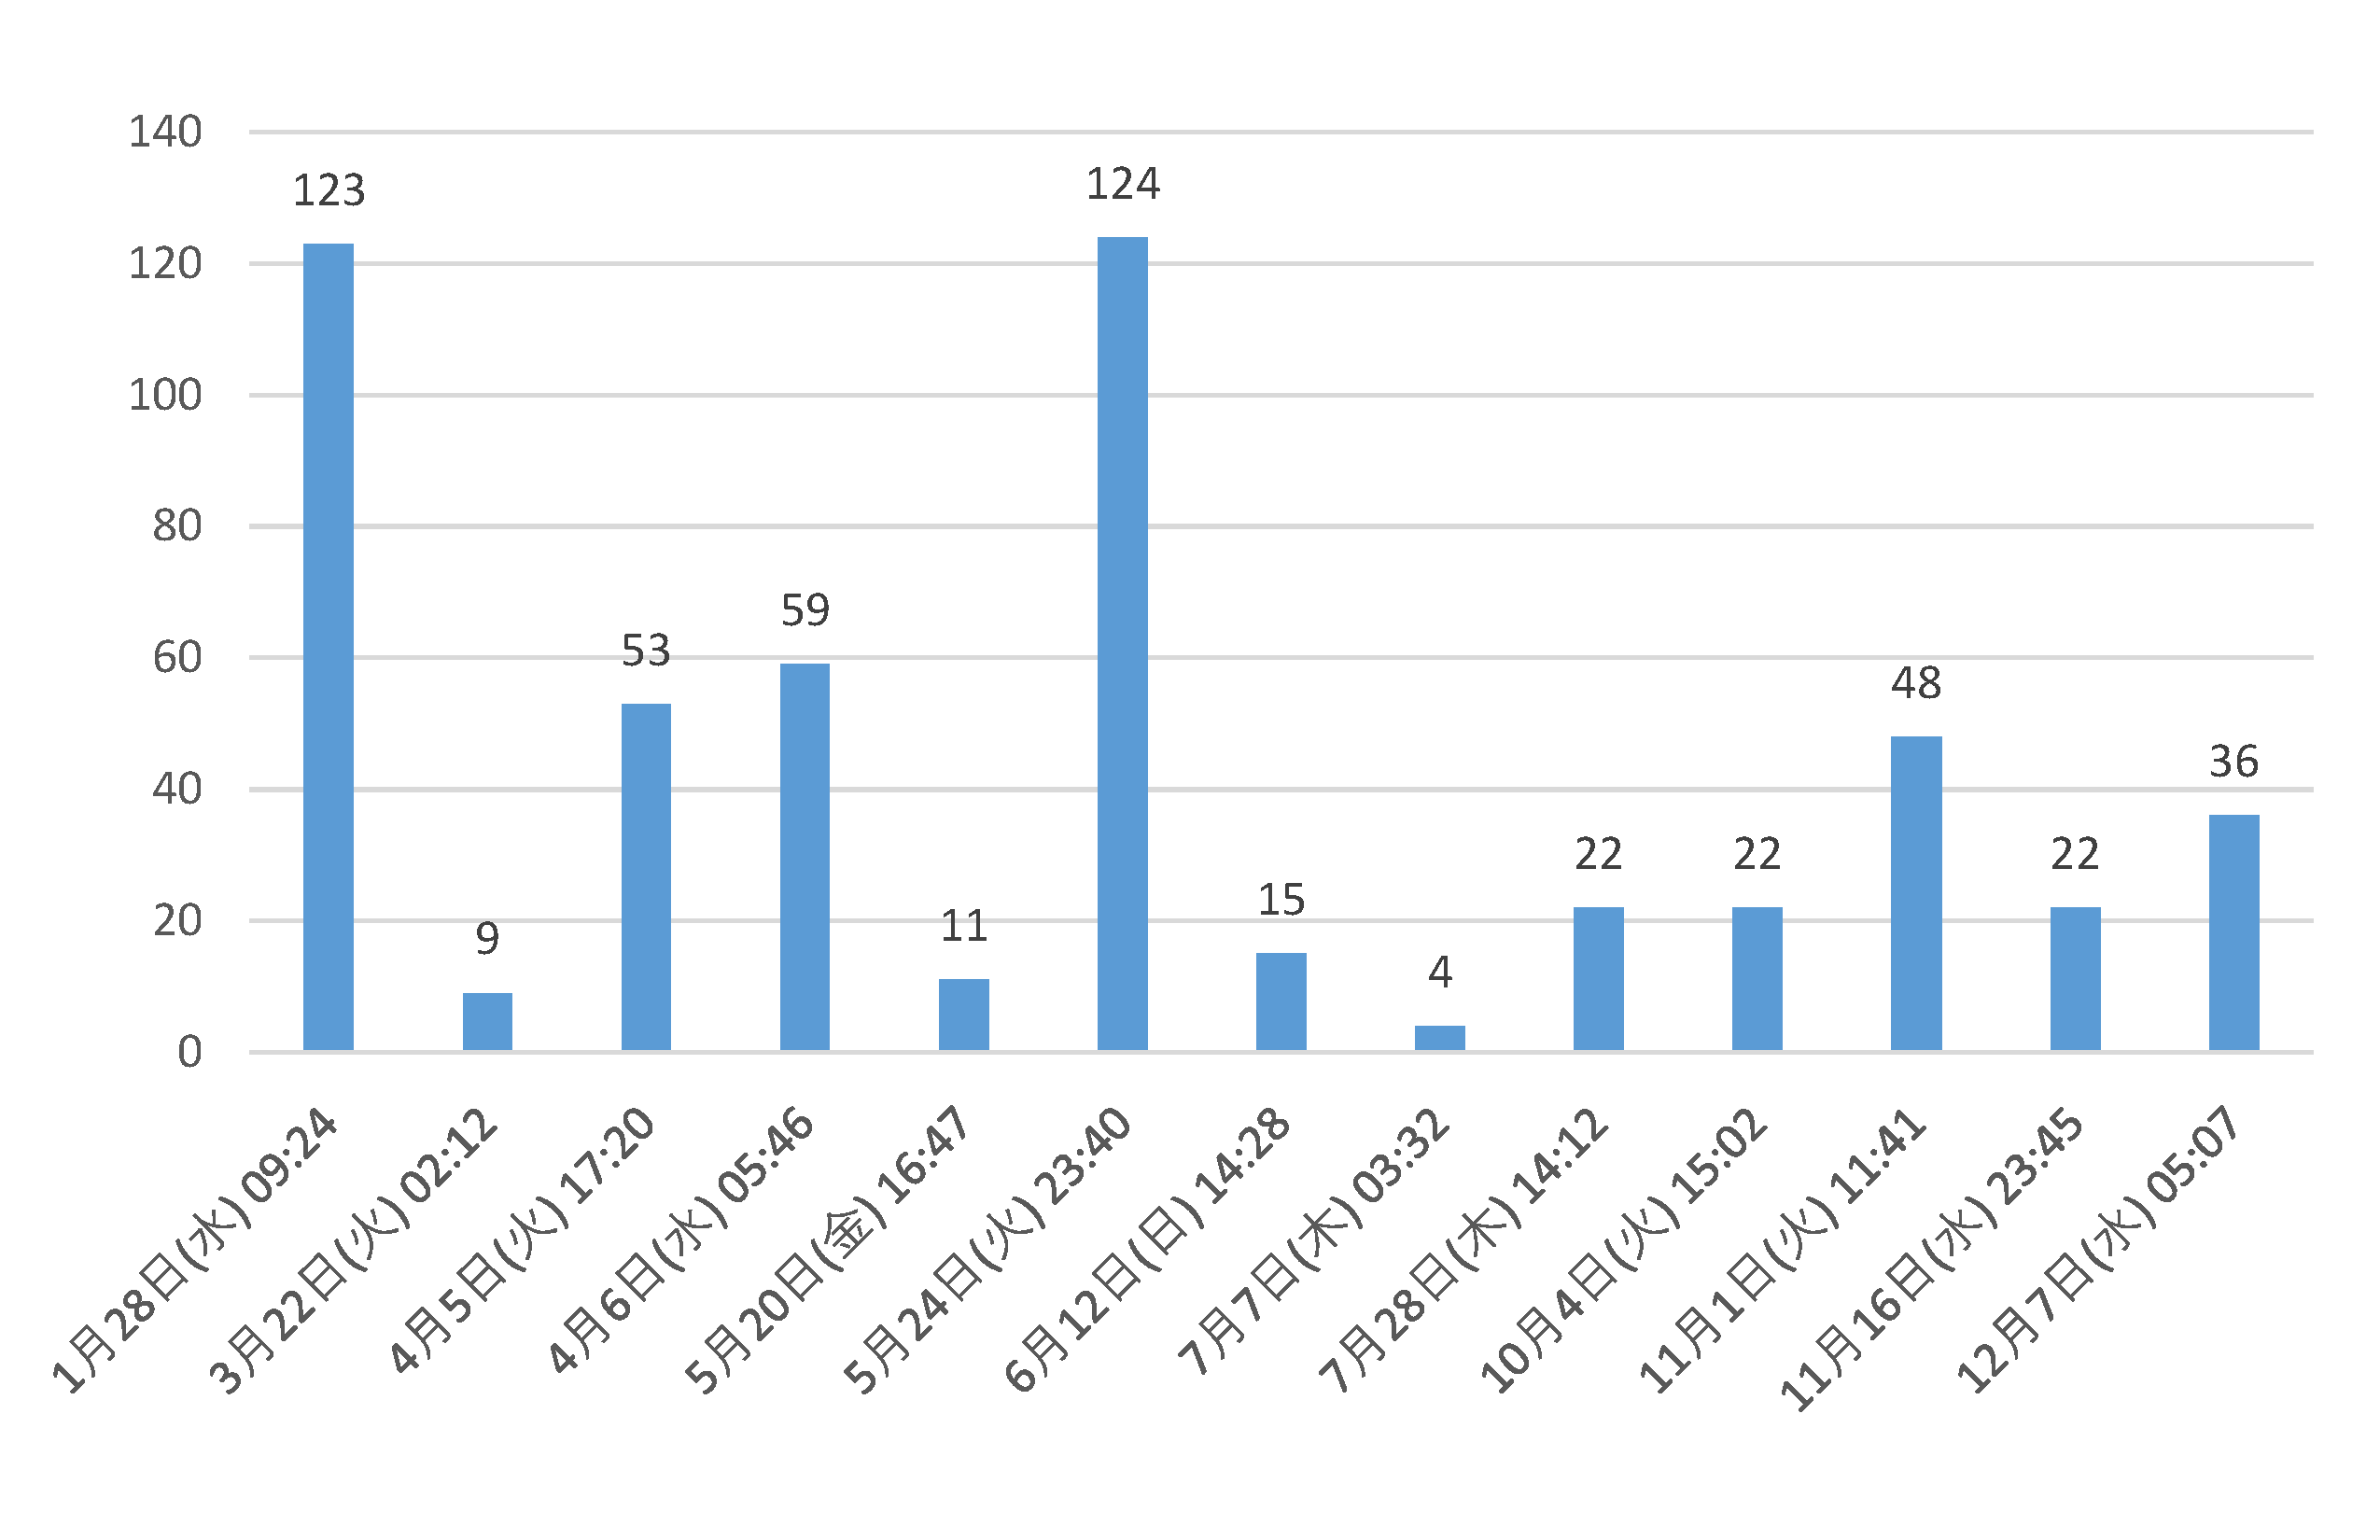
\includegraphics[width=8.4cm,clip]{graph1.pdf}
\caption{サービス停止から復旧までの間隔}\label{時間}
\end{figure}
\begin{figure}[H]
%\includegraphics[width=図の幅,clip]{ファイル名}\label{参照用ラベル}
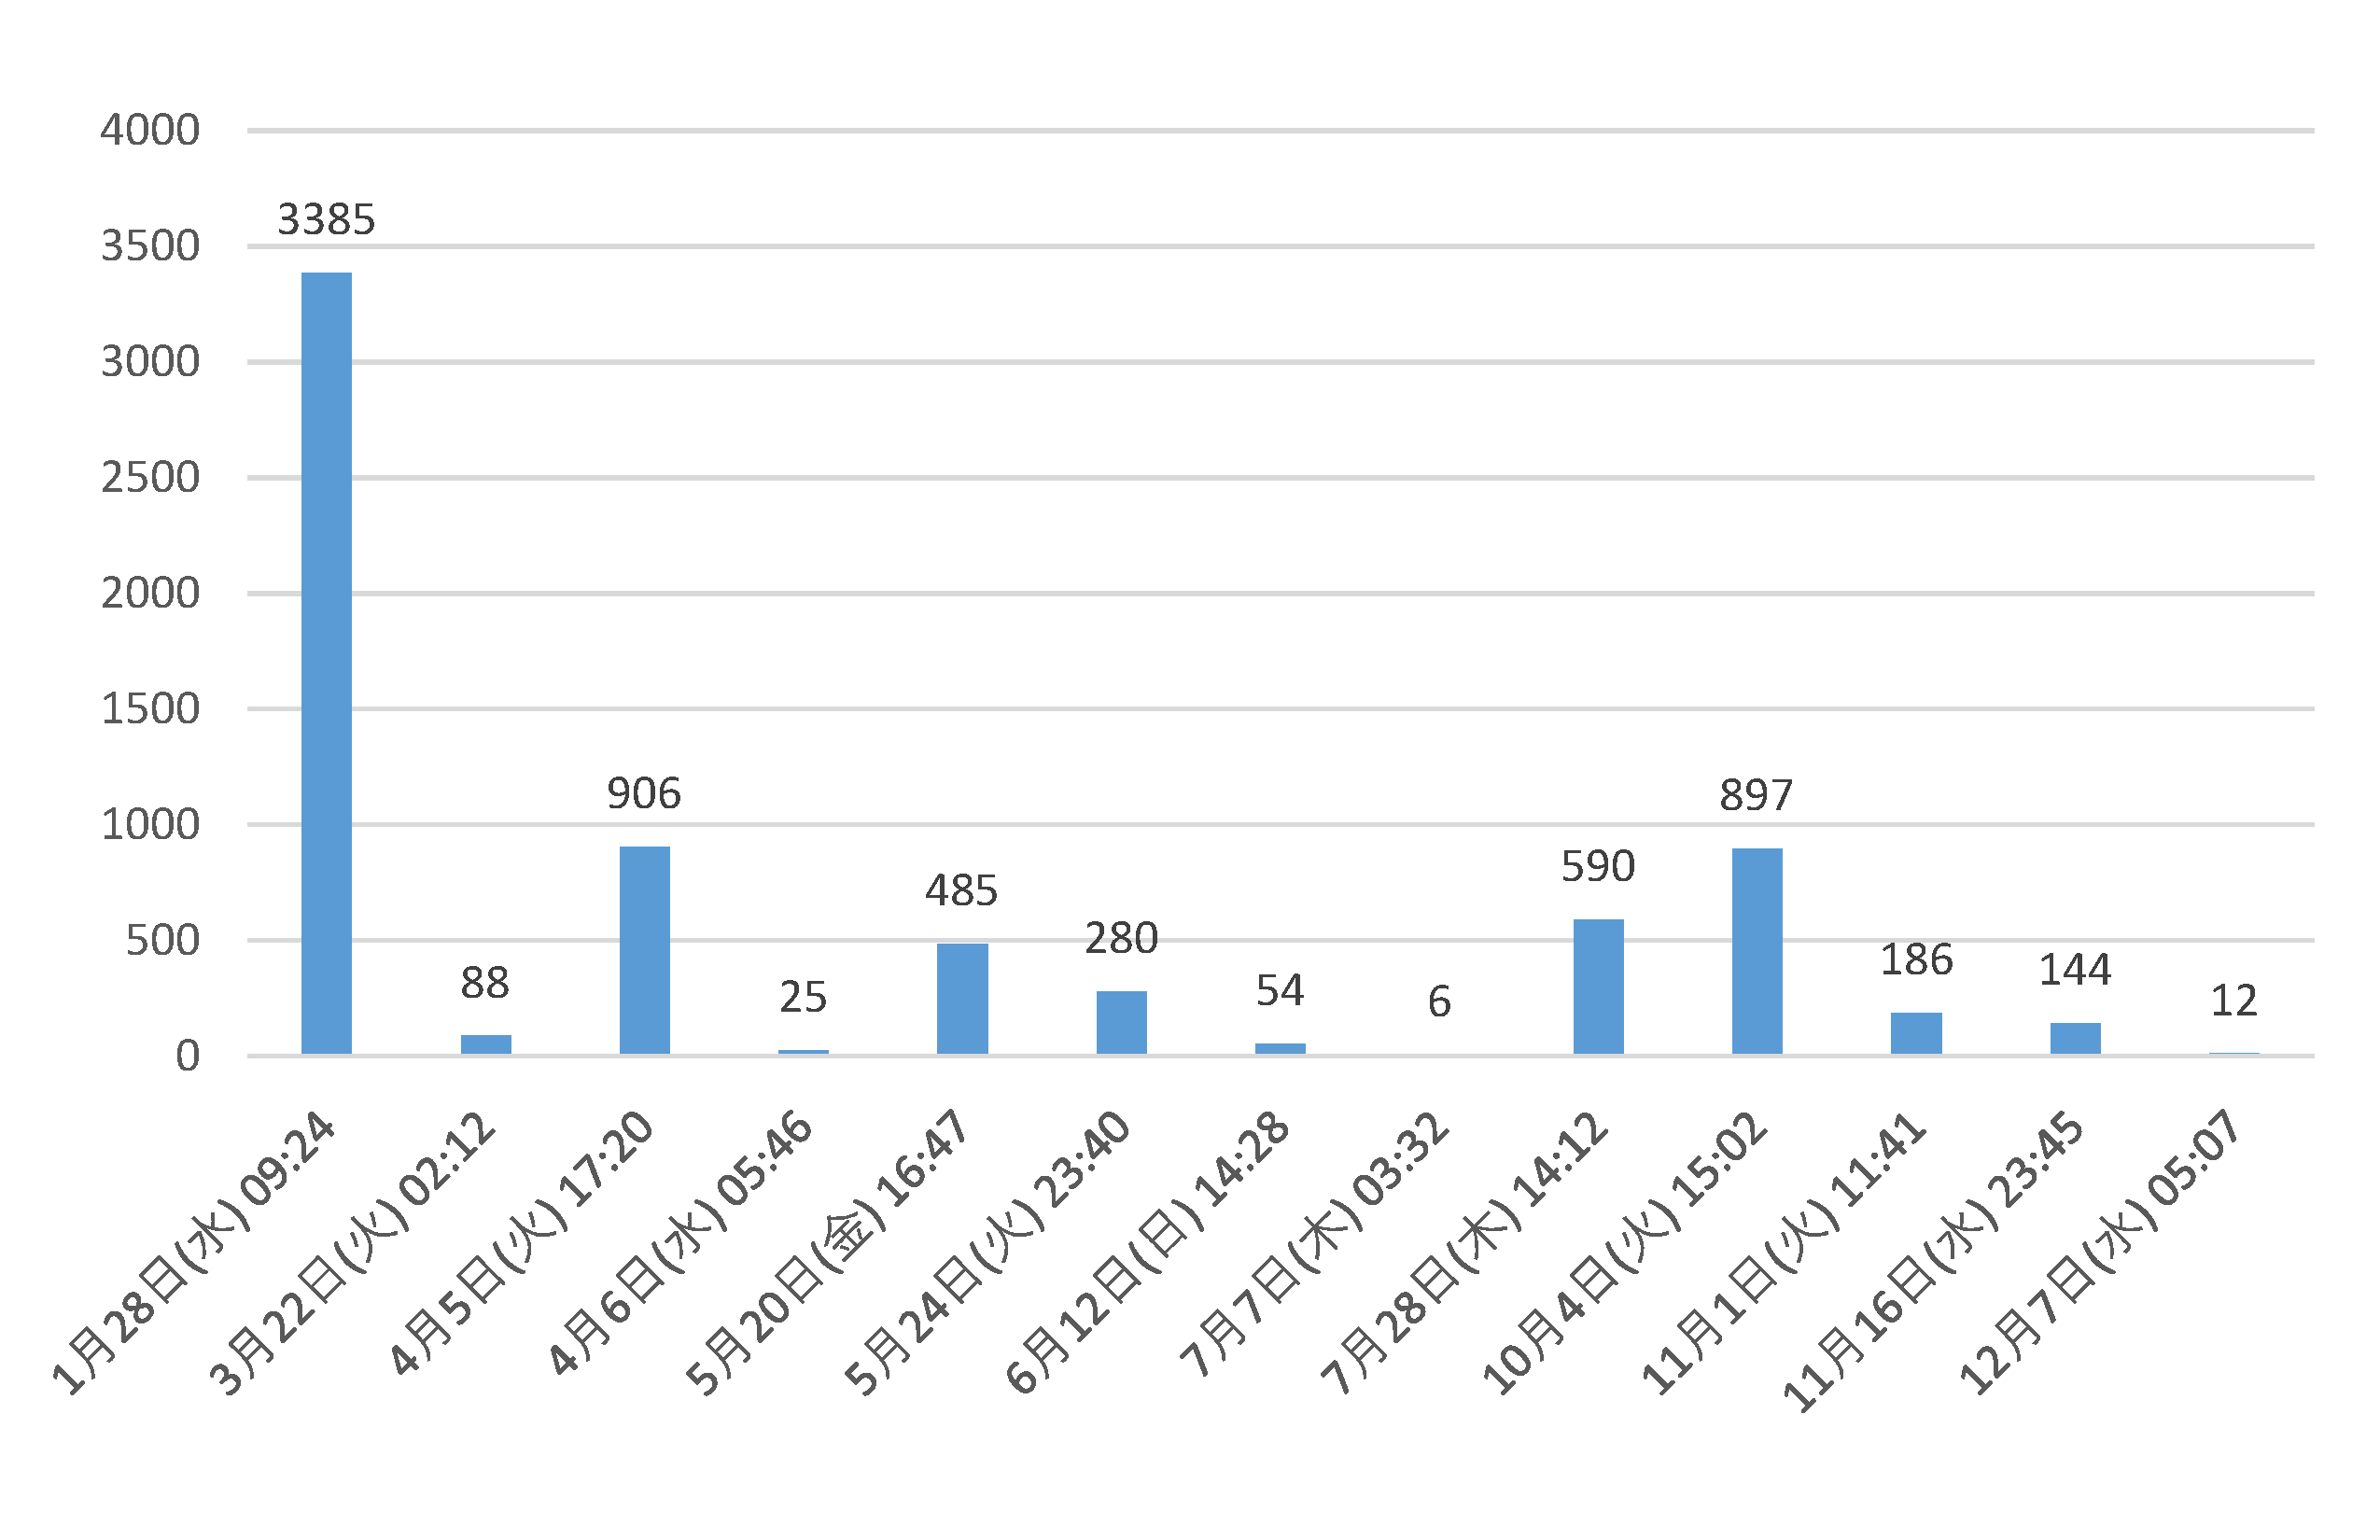
\includegraphics[width=8.4cm,clip]{graph2.pdf}
\caption{サービス停止中に投稿されたツイートの数}\label{ツイート数}
\end{figure}
13回分の各障害のサービス停止から復旧までの間隔を分単位でグラフにしたものが図\ref{時間}である.

そして,各障害のサービス停止中に投稿されたツイート数をグラフにしたものが図\ref{ツイート数}である.

\section{考察}
調査した13回分の障害を比較してみると,サービス停止から復旧までの間隔が同じくらいでも,1日の時間帯によってツイート数に違いがあった.特にツイート数が多かったのは平日の日中で,中でも会社への出勤や退勤にあたる時間帯であった.この時間帯にWebサービスが停止してしまうと例え数分の停止でもツイート数が多く,1日のタスクが確認できなかったり,チーム内でのコミュニケーションが取れなかったりする.

平日の日中であればツイート数が多いのは勿論だが,3月22日(火)の深夜2時台に発生した約9分間の障害でも88件のツイートが集まった.日中の障害でも6月12日(日)と7月28日(木)では同じ14時台の障害で停止時間に約7分の差はあるが500ツイート以上の差があった.これは日曜日に起きた障害であり,普段仕事をしている人々が休暇中であったため少なかったのではないかと考えられる.

また,GitHub StatusのStatus Messageを参照してツイート取得する日を決定していたが,Status Messageに記されているサービス停止や復旧のアナウンスよりも,サービス停止や復旧したという旨のツイートの方が平均して約 8 分ほど早かった.これはTwitterの速報性が優れていると言える.

\section{結論}
本研究ではWebサービスの障害発生について調査した.Webサービスは利便性が高く,それだけに依存してしまうこともある.そのサービスが停止することは頻繁に有ることではなく,一時的なものだが,そのWebサービスを使用しているユーザーの仕事やコミュニケーションに少なからず影響を及ぼす.したがって,ソフトウェア開発プロジェクトなどでWebサービスを使用する場合は,サーバーダウン等の障害が発生するリスクを考慮する必要がある.

\bibliographystyle{junsrt}
\bibliography{biblio}%「biblio.bib」というファイルが必要.


\end{document}